\documentclass[11 pt, a4paper]{article}
\usepackage[left=1.5cm,top= 1.5cm,right= 1.5cm,bottom=1.5cm]{geometry}
\usepackage[spanish]{babel}
\usepackage{amsthm}
\usepackage{graphicx}
\theoremstyle{definition}
\newtheorem{definicion}{Definici\'on}[section]
\graphicspath{{img/}}
\usepackage[utf8]{inputenc} 
\usepackage{amsmath,amssymb,amsfonts,latexsym} %Soporte para símbolos y font matemáticos
\usepackage{float}
\usepackage{amsthm}
\usepackage{enumerate}
% \usepackage[options]{algorithm2e}
\DeclareGraphicsExtensions{.pdf,.png,.jpg}
\DeclareGraphicsRule{.wmf}{bmp}{}{}
\newtheorem{no}{Nota}
\author{Trinidad Hern\'andez Norma Ver\'onica \\
        Vilchis Dom\'inguez Miguel Alonso}
\title{Tarea 2}
\date{}
\begin{document}
\maketitle

\section{Ejercicios}

\begin{enumerate}
 \item \textbf{Demostrar si las siguientes funciones son $\theta(n^2)$}
 \no Sea $f(n)$ una función por definición si $f(n) \in \theta(g(n))$ 
 implica que $ \exists c_1, c_2 \in \mathbb{N} $ y $\exists n_0 \in \mathbb{N}$ 
 tales que $0 \leq c_1*g(n) \leq f(n) \leq c_2*g(n)$.
 \begin{enumerate}
  \item $60n^2 + 5n +1$\\
  Por demostrar que $60n^2 + 5n +1 \in \theta(n^2)$. Por la \textbf{Nota 1}
  implica mostrar las constantes tales que la función queda acotada por 
  $n^2$ al multiplicarla por dichas constantes. Es decir:\\
  \begin{equation} 
   c_1* n^2 \leq 60n^2 + 5n +1 \leq c_2 * n^2 
   \end{equation}
  Sii
  \[ c_1 \leq 60 + \frac{5}{n} + \frac{1}{n^2} \leq c_2 \]
  Se propone $n_0 = 10$, $c_1 = 59$, $c_2 = 70$  Por lo que
  \[ 59 \leq 60 + \frac{5}{10} + \frac{1}{100} = \frac{6051}{100} \leq 70  \]
  Con lo que se sigue cumpliendo la desigualdad. Para finalizar la demostración 
  basta con mostrar que la desigualdad se sigue cumpliendo para
  $n > n_0$ con $n \in \mathbb{N}$.\\ 
  En efecto, para hacer una buena aproximación de lo que ocurre con 
  $n$ grandes, tomamos el $lim_{n \rightarrow \infty}$. Es decir:
  \[ lim_{n \rightarrow \infty} (60 + \frac{5}{n} + \frac{1}{n^2} )\]
   \[  = lim_{n \rightarrow \infty} 60 + lim_{n \rightarrow \infty} \frac{5}{n} + lim_{n \rightarrow \infty} \frac{1}{n^2} \]
  \[  = 60 + 0+0 \]
  Con lo que, se sigue cumpliendo la desigualdad $(1)$
  \begin{figure}[H]
         \centering
          %trim left bottom right top
          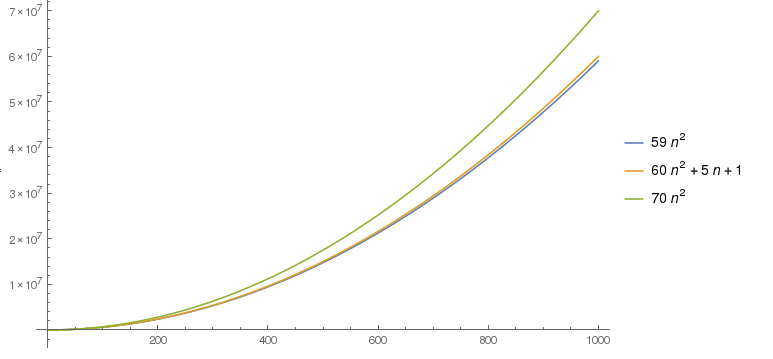
\includegraphics[trim=0cm 0cm 0cm 0cm, width=15cm]{inciso1.png} 
          \caption{Gráfica que muestra la comparación entre las funciones}
      \end{figure}
  \item $2n^2 - 16 n + 35$\\
  Siguendo un procedimiento parecido al inciso a, lo que haremos 
  para mostrar que $2n^2 - 16 n + 35 \in \theta(n^2)$ será utilizar 
  la definición que se dio en la \textbf{Nota 1}, por lo que:
  \begin{equation}
   c_1*n^2 \leq 2n^2 - 16 n + 35 \leq c_2*n^2
  \end{equation}
  Sii
  \[c_1 \leq 2 - \frac{16}{n} + \frac{35}{n^2} \leq c_2 \]
  Se propone $n_0 = 16$, $c_1 = 1$ y $c_2 = 3$ obteniendo:x
  
  \[ 1 \leq 2 - \frac{16}{10} + \frac{35}{256} = \frac{281}{256}\leq 3 \]
  Tomando el límite cuando $n$ tiende a infinito, para mostrar que la 
  desigualdad se cumple para  $n_0 < n \in \mathbb{N}$
  \[
   lim_{n \rightarrow \infty} 2 - \frac{16}{n} + \frac{35}{n^2}\]
   \[= lim_{n \rightarrow \infty} 2 - lim_{n \rightarrow \infty} \frac{16}{n} + lim_{n \rightarrow \infty} \frac{35}{n^2}\]
   \[= 2 - 0 +0   \]
  Con lo que se conserva la desigualdad $(2)$
    \begin{figure}[H]
         \centering
          %trim left bottom right top
          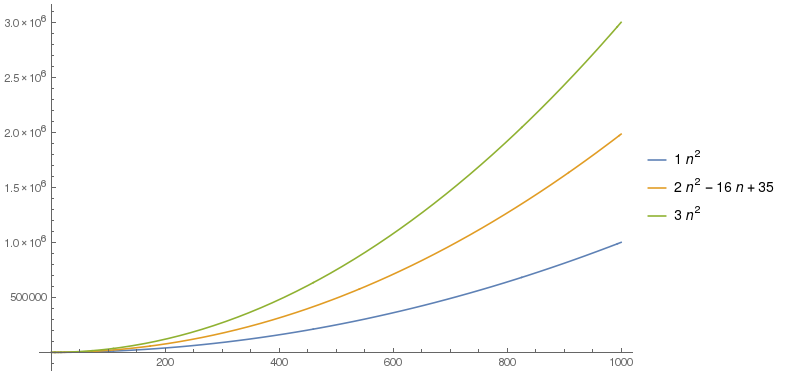
\includegraphics[trim=0cm 0cm 0cm 0cm, width=15cm]{inciso2.png} 
          \caption{Gráfica que muestra la comparación entre las funciones}
      \end{figure}
   \item $3 n^2 + 2* n\ ln\ n$
  Por demostrar que $3 n^2 + 2* n\ ln\ n \in \theta (n^2) $, en efecto:
  \begin{equation}
      c_1*n^2 \leq 3 n^2 + 2 * n\ ln\ n\leq c_2*n^2
  \end{equation}
  Sii
  \[  c_1\leq 3 + \frac{2 * \ ln\ n} {n}\leq c_2\]
  Si proponemos $n_0 = 128$, $c_1= 2$ y $c_2 = 4 $ obtenemos:
  \[ 2 \leq  3 + \frac{2 * \ ln\ 128} {128} = 3 + \frac{7}{64}= \frac{199}{64} \leq 4 \]
 Para demostrar que la desigualdad $(3)$ se cumple para $n_0 < n \in \mathbb{N}$
 tomamos $lim_{n \rightarrow \infty}$: 
 \[lim_{n \rightarrow \infty} 3 + \frac{2 * \ ln\ n} {n}\]
  \[= 3 +  lim_{n \rightarrow \infty} \frac{2 * \ ln\ n} {n}\]
 \[ = 3 +0 \]
 Con lo que la desigualdad $(3)$ se conserva.
   \begin{figure}[H]
         \centering
          %trim left bottom right top
          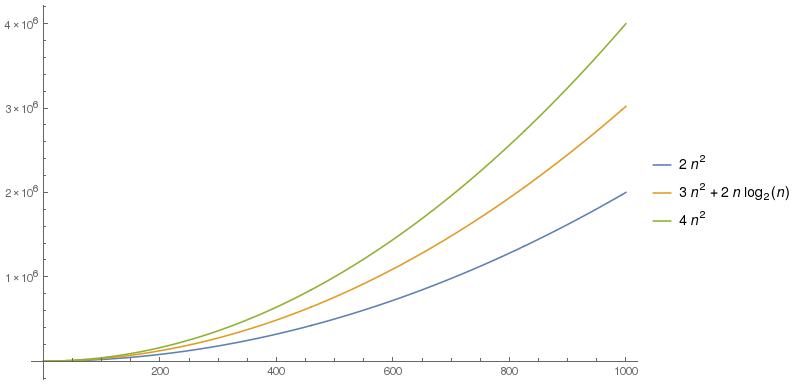
\includegraphics[trim=0cm 0cm 0cm 0cm, width=15cm]{inciso3.png} 
          \caption{Gráfica que muestra la comparación entre las funciones}
      \end{figure}



  
  
  \item $2+4+6+ ... + 2n$
  
  \item $For\ i = 1 \ to \ n$\\
        $.\ \ \ \ For\ j = 1 to i$\\
        $.\ \ \ \ \ \ \ \ For\ x = 1 to i$ \\
        $.\ \ \ \ \ \ \ \ \ \ \ \ x= x +1$ \\                     

 \end{enumerate}

\end{enumerate}
\end{document}

